\chapter{El caso infinito}
\label{chap:inf}
\noindent
Sea $\vec{p} \in \R^n$ un vector esencialmente entero y recordemos de la definición
\ref{theory:def:rational} que tiene un único múltiplo coprimo $\vec{q} \in \Z^n$. Es decir, existe
un único escalar $m \in \R$ que satisface tres cosas: $\vec{p} = m\vec{q}$, las entradas $q_1,
\ldots, q_n$ son coprimas, y la primera entrada no nula $q_i$ es positiva. Supondremos, sin pérdida
de generalidad, que $m$ es positivo.

Retomemos el entero $\eta \in \Z$ del lema \ref{phase-1:lemma:eta} que parametriza la primera capa
entera que satisface el presupuesto \eqref{theory:constraint:budget}. A causa del teorema
\ref{theory:th:feasibility}, sabemos que si $q_i < 0$ para alguna $i \in \braces{1, \ldots, n}$,
entonces la $\eta$-ésima capa entera contiene un número infinito de puntos factibles.

\begin{corollary}
	\label{cor:inf:obj}
	Supongamos que $q_i < 0$ para algún $i \in \braces{1, \ldots, n}$. Entonces el valor óptimo del
	programa lineal entero (\ref{theory:formulation}) es $m\eta$. Además, si $m$ es positivo,
	tenemos que $\eta$ es el múltiplo de $m$ más grande que satisface $m\eta \leq u$, donde $u$ es
	el lado derecho de la restricción presupuestaria \eqref{theory:constraint:budget}.
\end{corollary}
\begin{proof}
	Por hipótesis, una entrada de $\vec{q}$ es negativa. Del segundo caso del teorema
	\ref{theory:th:feasibility} sabemos que existen una infinidad de soluciones en la $\eta$-ésima
	capa entera, así que sea $\vec{x}^*$ una de ellas. Por el lema \ref{theory:lemma:utility} se
	sigue que $\vec{q}^T\vec{x}^* = \eta$, pero $\vec{p} = m\vec{q}$ por la definición
	\ref{theory:def:rational}, por lo que obtenemos $\vec{p}^T\vec{x}^* = m\vec{q}^T\vec{x}^* =
	m\eta$.

	Ahora bien, supongamos $m$ es positivo pero que $\eta$ no es el múltiplo más grande de $m$ que
	satisface $m\eta \leq u$. Supongamos que $\xi \in \Z$ satisface $m\xi \leq u$ y también $\eta <
	\xi$. Por el lema \ref{phase-1:lemma:eta} tenemos $\eta = \floor{u/m}$. Luego,
	\begin{equation*}
		m\eta = m\left\lfloor \frac{u}{m} \right\rfloor < m\xi \leq u
		\implies \left\lfloor \frac{u}{m} \right\rfloor < \xi \leq \frac{u}{m},
	\end{equation*}
	pero esto contradice las propiedades de la función piso. Finalmente, por hipótesis tenemos que
	$m$ es positivo y por lo tanto $\eta$ debe ser el múltiplo más grande de $m$ que satisface
	$m\eta \leq u$.
\end{proof}

\begin{observation}
	Para ilustrar la conveniencia de restringir $m$ a que sea positivo, consideremos el caso cuando
	$m < 0$. Del lema \ref{phase-1:lemma:eta} tenemos que $\eta \coloneq \lceil u/m \rceil$
	parametriza también la primera capa entera que satisface el presupuesto, pues ahora tenemos de
	la restricción \eqref{theory:constraint:budget} que $\vec{p}^T\vec{x} \leq u$ si y solo si
	$\vec{q}^T\vec{x} \geq u/m$. Se sigue cumpliendo que el valor óptimo del problema
	\eqref{theory:formulation} es $m\eta$. Sin embargo, $\eta$ ahora es el múltiplo más pequeño de $m$
	que satisface $m\eta \geq u$.
\end{observation}

Puesto que somos capaces de decidir si un escalar $u^*$ es el valor óptimo del problema
\eqref{theory:formulation}, nos preguntamos ahora cómo obtener la solución óptima.

Por hipótesis de este capítulo, el vector coprimo $\vec{q}$ tiene al menos una entrada negativa. Del
segundo caso del teorema \ref{theory:th:feasibility}, sabemos que las infinitas soluciones de
\eqref{theory:formulation} se encuentran en la $\eta$-ésima capa entera. Luego, del lema
\ref{theory:lemma:utility} tenemos que estas soluciones satisfacen la ecuación lineal diofantina
$\vec{q}^T\vec{x} = \eta$.

Supongamos, por el momento, que $\vec{q}$ no tiene entradas nulas. Podemos permutar las entradas de
$\vec{q}$ sin afectar la el problema \eqref{theory:formulation}. En efecto, toda solución $\vec{x}
\in \Z^n$ de \eqref{theory:formulation} es no negativa y satisface $\vec{q}^T\vec{x} = \eta$. Sea $P
\in \Z^{n \times n}$ una matriz de permutación. Observemos que $\vec{x}$ es no negativo si y solo si
$P\vec{x}$ es no negativo. Además,
\begin{equation*}
	\eta = \vec{q}^T\vec{x} = \vec{q}^TP^TP\vec{x} = (P\vec{q})^T(P\vec{x}).
\end{equation*}
Por lo que podemos encontrar una solución entera no negativa $\vec{x}$ de la ecuación lineal
diofantina $(P\vec{q})^T\vec{x} = \eta$ y entonces $P\vec{x}$ es solución de
\eqref{theory:formulation}.

\begin{observation}
	Si $\vec{q} \in \Z^n$ es un vector coprimo, entonces $P\vec{q}$ no necesariamente lo es, ya que
	posiblemente $(P\vec{q})_1 < 0$. Esto no constituye un problema, pues la construcción de soluciones
	en la sección \ref{subsec:dioph-eq} requiere que las entradas del vector sean coprimas y no hace
	suposiciones sobre sus signos.
\end{observation}

En particular podemos suponer, sin pérdida de generalidad, que las entradas de  $\vec{q}$ satisfacen
$q_{n-1} < 0 < q_n$. Como $\vec{q}$ no tiene entradas nulas, de la
definición \ref{theory:def:rational} sabemos que $q_1$ es positivo y, por suposición de este capítulo,
alguna entrada $q_j$ es negativa, así que podemos permutar estas entradas con las de $q_n$ y
$q_{n-1}$, respectivamente.

De la proposición \ref{prop:xint} sabemos que el conjunto de soluciones enteras de la ecuación
lineal diofantina $\vec{q}^T\vec{x} = \eta$ es $\braces{\eta\vec{\nu} + M\vec{t} \vcentcolon \vec{t}
\in \Z^{n-1}}$. Así pues, basta encontrar condiciones suficientes en $\vec{t}$ para asegurar la no
negatividad de la solución $\vec{x} \coloneq \eta\vec{\nu} + M\vec{t}$.

Para que las primeras $n - 2$ entradas de $\vec{x}$ sean no negativas, debe ser el caso que $t_i \in
\Z$ satisfaga \eqref{eq:param-lb} para todo $1 \leq i \leq n - 2$. Recuperamos de
\eqref{eq:last-solution} que las últimas dos entradas de $\vec{x}$ son
\begin{equation*}
	\begin{cases}
		x_{n-1} = \omega_{n-1}x_{n-1}' + \frac{q_n}{\prod_{j=1}^{n-1}g_j}t_{n-1}, \\
		x_n = \omega_{n-1}x_n' - \frac{q_{n-1}}{\prod_{j=1}^{n-1}g_j}t_{n-1},
	\end{cases}
\end{equation*}
donde los enteros $g_i$ están definidos por \eqref{dummy:next-g} con $g_1 = 1$, $\omega_{n-1}$ está
definida a través de la relación de recurrencia \eqref{eq:omega-recurrence} con condición inicial
$\omega_1 = \eta$, y $x_{n-1}', x_n'$ son coeficientes de Bézout que satisfacen
\eqref{eq:last-equation-bez}. Definamos, por conveniencia,
\begin{equation}
	\label{eq:lr-bounds}
	b_1 \coloneq -\frac{\omega_{n-1}x_{n-1}'}{q_n} \cdot \prod_{j=1}^{n-1}g_j, \quad
	b_2 \coloneq \frac{\omega_{n-1}x_{n}'}{q_{n-1}} \cdot \prod_{j=1}^{n-1}g_j.
\end{equation}
Puesto que $q_{n-1} < 0 < q_n$, si despejamos $t_{n-1}$ de \eqref{eq:last-solution} encontramos que
las últimas dos entradas de $\vec{x}$ son no negativas si y solo si $t_{n-1}$ satisface
\begin{equation}
	\label{eq:feasible-param:collapsed}
	t_{n-1} \geq \ceil{\max\lbrace b_1, b_2 \rbrace}.
\end{equation}

El siguiente lema fortalece nuestros resultados al generalizarlo para todo lado derecho de
\eqref{eq:dioph}.
\begin{lemma}
	\label{lemma:t-existence}
	Sea $\vec{p} \in \R$ un vector esencialmente entero, y supongamos que su múltiplo coprimo
	$\vec{q} \in \Z^n$ tiene entradas no nulas y al menos una de ellas es negativa. Entonces la
	ecuación lineal diofantina \eqref{eq:dioph} tiene una infinidad de soluciones enteras no
	negativas.
\end{lemma}
\begin{proof}
	Supongamos, sin pérdida de generalidad, que $q_{n-1} < 0 < q_n$. Sea $\vec{t} \in \Z^{n-1}$ tal
	que
	\begin{equation*}
		t_i \geq \begin{cases}
			\ceil{-\frac{\omega_ix_i'}{g_{i + 1}}}, & i < n - 1, \\[0.5em]
			\ceil{\max\lbrace b_1, b_2 \rbrace}, & i = n - 1,
		\end{cases}
	\end{equation*}
	y sea
	\begin{equation*}
		\vec{x} \coloneq k\vec{\nu} + M\vec{t},
	\end{equation*}
	donde recuperamos $\vec{\nu}$ y $M$ de \eqref{eq:vec-omega} y \eqref{eq:mat-T}, respectivamente.
	De la proposición \ref{prop:xint}, así como de \eqref{eq:param-lb} y
	\eqref{eq:feasible-param:collapsed}, se sigue que $\vec{x}$ es entero y no negativo. Finalmente,
	de los lemas \ref{lemma:iso1} y \ref{lemma:iso2} encontramos que
	\begin{equation*}
		\vec{q}^T\vec{x} = k\vec{q}^T\vec{\nu} + \vec{q}^TM = k,
	\end{equation*}
	por lo que $\vec{x}$ es solución de \eqref{eq:dioph}.
\end{proof}

En la práctica es mejor usar la relación de recurrencia \eqref{eq:recurrence} y ``construir'' las
entradas $x_i$ al mismo tiempo que definimos $t_i$ de manera que satisfaga \eqref{eq:param-lb} y
\eqref{eq:feasible-param:collapsed}. Si procedemos de esta forma no tenemos que encontrar primero
$\vec{\nu}$ y $M$, determinar $\vec{t}$ y luego recuperar $\vec{x}$.

El algoritmo \ref{algo:inf} (pág.~\pageref{algo:inf}) muestra aquel procedimiento constructivo.
Para ello, suponemos la existencia de una subrutina \texttt{Bezout} que, como su nombre lo indica,
calcula los coeficientes de Bézout entre dos enteros. El autor reitera, así como lo hizo en la
sección \ref{section:number-theory}, que estos coeficientes se pueden calcular por medio del
algoritmo extendido de Euclides.

\begin{algorithm}[ht]
	\LinesNumbered
	\DontPrintSemicolon
	\SetKwProg{Fn}{Fn}{\string:}{}
	\SetKwFunction{Bezout}{Bezout}
	\SetKwFunction{NonNegativeIntSol}{NonNegativeIntSolInf}
		\KwData{\\
			$\vec{q} \in \Z^n$ con entradas coprimas no nulas y tal que $q_{n-1} < 0 < q_n$. \\
			$\eta \in \Z_{\geq 0}$.
			}
		\KwResult{\\
			$\vec{x} \in \Z^n_{\geq \vec{0}}$ tal que $\vec{q}^T\vec{x} = \eta$.
		}
		\Begin{
			$\vec{x} \leftarrow \vec{0}$\;
			$\omega_1 \leftarrow \eta$\;
			$p \leftarrow 1$\;
			\For{$i \leftarrow 1$ \KwTo $n - 2$\label{alg:def:inf:loop}}{
				$g_{i+1} \leftarrow \gcd{q_{i+1} / p, \ldots, q_n / p}$\quad\tcp*[h]{ecuación
				\eqref{dummy:next-g}}\; \label{alg:def:inf:g}
				$x_i', \omega_{i+1}' \leftarrow$ \Bezout{$q_i / p$, $g_{i+1}$}\; \label{alg:def:inf:bez}
				$t_i \leftarrow \ceil{-\omega_i x_i' / g_{i+1}}$\quad\tcp*[h]{ecuación
				\eqref{eq:param-lb}}\; \label{alg:def:inf:t}
				\tcp*[h]{ecuación \eqref{eq:recurrence}}\;
				$x_i \leftarrow \omega_i x_i' + g_{i+1}t_i$\; \label{alg:def:inf:x}
				$\omega_{i+1} \leftarrow \omega_i \omega_{i+1}' - q_i t_i / p$\; \label{alg:def:inf:w}
				\tcp*[h]{actualizar producto}\;
				$p \leftarrow pg_{i+1}$\;
			}

			$x_{n-1}', x_n' \leftarrow$ \Bezout{$q_{n-1} / p$, $q_n / p$}\; \label{alg:def:inf:lastw}
			\tcp*[h]{ecuación \eqref{eq:lr-bounds}}\;
			$b_1 \leftarrow -\omega_{n-1} x_{n-1}' \cdot p/ q_n$\;
			$b_2 \leftarrow \omega_{n-1} x_n' \cdot p/ q_{n-1}$\;
			$t_{n-1} \leftarrow \ceil{\max\lbrace b_1, b_2\rbrace}$\quad\tcp*[h]{ecuación
			\eqref{eq:feasible-param:collapsed}}\;
			\tcp*[h]{ecuación \eqref{eq:last-solution}}\;
			$x_{n-1} \leftarrow \omega_{n-1}x_{n-1}' + q_nt_{n-1} / p$\;
			$x_{n} \leftarrow \omega_{n-1}x_{n}' - q_{n-1}t_{n-1} / p$\;

			\Return{$\vec{x}$}\;
		}
	\caption{\texttt{NonNegativeIntSolInf}}
	\label{algo:inf}
\end{algorithm}

\begin{lemma}
	\label{lemma:alg:inf:correct}
	El algoritmo \ref{algo:inf} es correcto.
\end{lemma}
\begin{proof}
	Basta observar que el algoritmo sigue la construcción recursiva de la sección
	\ref{subsec:dioph-eq}, donde escogemos las variables libres $t_i$ como lo indican
	\eqref{eq:param-lb} y \eqref{eq:feasible-param:collapsed} para asegurar que $\vec{x} \in \Z^n$
	sea no negativo.
\end{proof}

Ahora bien, supongamos que $\vec{q}$ tiene entradas nulas. Sea
\begin{equation*}
	I^\circ \coloneq \braces{i \vcentcolon q_i = 0},
\end{equation*}
y también definamos el vector $\tvec{q}$ cuyas entradas son las entradas no nulas de $\vec{q}$.
Supongamos que la penúltima entrada de $\tvec{q}$ es negativa y que su última entrada es positiva. A
causa del lema anterior, el algoritmo \ref{algo:inf} encuentra un vector $\tvec{x}$ entero no
negativo que satisface $\tvec{q}^T\tvec{x} = \eta$. Luego, encontramos que el vector $\vec{x}$ dado
por
\begin{equation*}
	x_i \coloneq
	\begin{cases}
		\tilde{x}_i, & i \not \in I^\circ, \\
		0, & i \in I^\circ,
	\end{cases}
\end{equation*}
es entero, no negativo, y también satisface $\vec{q}^T\vec{x} = \eta$.

El algoritmo \ref{algo:inf:ext} (pág.~\pageref{algo:inf:ext}) extiende el algoritmo \ref{algo:inf} en
el sentido que incorpora esta forma de manejar las entradas nulas de $\vec{q}$. Además, modifica el
vector $\tvec{q}$ de manera que aseguramos que su penúltima entrada es negativa y su última entrada
es positiva, por lo que podemos deshacernos de este supuesto. Al igual que en el algoritmo anterior,
suponemos la existencia de las subrutinas \texttt{length} y \texttt{switch}, las cuales determinan
la dimensión de un vector $\vec{q}$ y permutan sus entradas, respectivamente. Ambas subrutinas son
estándar en la literatura.

\begin{algorithm}[ht]
	\LinesNumbered
	\DontPrintSemicolon
	\SetKwProg{Fn}{Fn}{\string:}{}
	\SetKwFunction{switch}{switch}
	\SetKwFunction{NonNegativeIntSol}{NonNegativeIntSolInf}
	\SetKwFunction{FindNegEntry}{FindNegEntry}
	\SetKwFunction{length}{length}
	\SetKwFunction{Dioph}{Dioph}
		\KwData{\\
			$\vec{q} \in \Z^n$ coprimo con al menos una entrada negativa. \\
			$\eta \in \Z_{\geq 0}$.
			}
		\KwResult{\\
			$\vec{x} \in \Z^n_{\geq \vec{0}}$ tal que $\vec{q}^T\vec{x} = \eta$.
		}
		$\vec{x} \leftarrow \vec{0}$\;
		$\vec{\sigma} \leftarrow \left(i \colon q_i \neq 0\right)$\;
		$\tvec{q} \leftarrow \left( q_i \colon q_i \neq 0 \right)$\;
		\label{alg:def:inf:tilde-q}

		$m \leftarrow$ \length{$\tvec{q}$}\; \label{alg:subr:length}
		\switch{$\tvec{q}$, $1$, $m$}\quad\tcp*[h]{$\tvec{q}_m > 0$}\; \label{alg:subr:switch1}

		\For{$i \leftarrow 1$ \KwTo $m - 1$}{ \label{alg:inf:loop}
			\If{$\tilde{q}_i < 0$}{
				$j \leftarrow i$\;
				ir al paso \ref{alg:subr:switch3}\;
			}
		}
		\switch{$\tvec{q}$, $j$, $m - 1$}\quad\tcp*[h]{$\tvec{q}_{m-1} < 0$}\; \label{alg:subr:switch3}
		$\tvec{x} \leftarrow$ \NonNegativeIntSol{$\tvec{q}$, $\eta$}\quad\tcp*[h]{algoritmo
		\ref{algo:inf}}\;
		\switch{$\tvec{x}$, $j$, $m - 1$}\; \label{alg:subr:switch2}
		\switch{$\tvec{x}$, $1$, $m$}\;

		\For{$i \leftarrow 1$ \KwTo $m$}{ \label{alg:inf:loop2}
			$x_{\sigma_i} \leftarrow \tilde{x}_i$\;
		}
		\Return{$\vec{x}$}
	\caption{\texttt{Dioph}}
	\label{algo:inf:ext}
\end{algorithm}

\begin{theorem}
	\label{th:alg:inf}
	El algoritmo \ref{algo:inf:ext} es correcto.
\end{theorem}
\begin{proof}
	Primero mostramos que el vector $\tvec{q}$ satisface las hipótesis del algoritmo
	\ref{algo:inf}. Por definición, en la línea \ref{alg:def:inf:tilde-q}, tenemos que ninguna
	entrada de $\tvec{q}$ es nula.

	Recordemos de la definición \ref{theory:def:rational} que, como $\vec{q}$ es el múltiplo coprimo
	de un vector esencialmente entero $\vec{p}$, su primera entrada no nula es positiva. Así, es
	cierto que $\tilde{q}_1 > 0$. A partir de la transposición en la línea \ref{alg:subr:switch1}
	encontramos que $\tilde{q}_m > 0$.

	Del ciclo en la línea \ref{alg:inf:loop} recuperamos el primer índice $j$ tal que $\tilde{q}_j < 0$ y
	lo transponemos con la $(m - 1)$-ésima entrada de $\tvec{q}$ en la línea
	\ref{alg:subr:switch3}, de manera que obtenemos $\tilde{q}_{m-1} < 0$.

	Con los tres puntos anteriores, encontramos que el vector $\tvec{q}$ satisface las
	hipótesis del algoritmo \ref{algo:inf} y por lo tanto el vector $\tvec{x}$ es no negativo
	y satisface la ecuación lineal diofantina $\tvec{q}^T\tvec{x} = \eta$.

	Las siguientes dos líneas se encargan de invertir las transposiciones hechas previamente.
	Finalmente, en el ciclo de la línea \ref{alg:inf:loop2} insertamos en $\vec{x}$ las entradas $i$
	de $\tvec{x}$ donde $q_{\sigma_i} \neq 0$. En otro caso tenemos $x_i = 0$. Así pues, el vector
	$\vec{x} \in \Z^n$ es no negativo y también satisface
	\begin{equation*}
		\vec{q}^T\vec{x} = \sum_{i = 1}^{n}q_ix_i
		= \sum_{i = 1}^{m}q_{\sigma_i}x_{\sigma_i}
		= \sum_{i = 1}^{m}\tilde{q}_i\tilde{x}_i
		= \eta,
	\end{equation*}
	por lo que concluimos que el algoritmo \ref{algo:inf:ext} es correcto.
\end{proof}

\begin{theorem}
	\label{infinite:th:complexity}
	Sea $\vec{p} \in \R^n$ un vector esencialmente entero tal que su múltiplo coprimo $\vec{q} \in
	\Z^n$ tiene al menos una entrada negativa. Entonces el problema \eqref{theory:formulation} se
	puede resolver a través de encontrar la solución de una ecuación lineal diofantina en $n$
	incógnitas.
\end{theorem}
\begin{proof}
	Como $\vec{q}$ es el múltiplo coprimo de $\vec{p}$, existe un escalar $m$ tal que
	$\vec{p} = m\vec{q}$. Supongamos, sin pérdida de generalidad, que $m$ es positivo. Recuperemos
	$\eta$ del lema \ref{phase-1:lemma:eta}. Por hipótesis, una entrada de $\vec{q}$ es negativa, y
	entonces este vector satisface las condiciones del algoritmo \ref{algo:inf:ext}. Por el teorema
	\ref{th:alg:inf} podemos encontrar, a partir de resolver solo una ecuación lineal diofantina, un
	vector entero no negativo $\vec{x}$ que satisface $\vec{q}^T\vec{x} = \eta$. Observemos que
	\begin{equation*}
		\vec{p}^T\vec{x} = m\vec{q}^T\vec{x} = m\eta.
	\end{equation*}
	Por el corolario \ref{cor:inf:obj} concluimos que $\vec{x}$ no solo es factible para el problema
	\eqref{theory:formulation}, sino que también es un punto óptimo.
\end{proof}

\section{Experimentos numéricos}
\label{sec:inf:exp}
\noindent
En esta subsección exponemos la dependencia implícita que tiene Ramificación y Acotamiento (R\&A)
con la precisión numérica que usamos para especificar el vector objetivo en programas lineales
enteros. Por lo tanto, no es cierto que estos programas dependan exclusivamente de su dimensión y de
su número de restricciones, como se escucha normalmente.

En primer lugar, determinamos la complejidad algorítmica del algoritmo \ref{algo:inf:ext} y lo
usamos como base de nuestras comparaciones. En segundo lugar, enseñamos por qué el método de R\&A
también depende del número de decimales usados para especificar las entradas del vector objetivo. En
tercer lugar, diseñamos un experimento numérico que ilustre esta dependencia.

\subsection{Análisis de nuestro método}
\label{subsec:inf:complex}
\noindent
En ambos algoritmos \ref{algo:inf} y \ref{algo:inf:ext} suponemos que el costo de realizar
operaciones aritméticas es constante. Primero analizamos el algoritmo \ref{algo:inf}. En el ciclo de
la línea \ref{alg:def:inf:loop} realizamos $\mathcal{O}(n)$ multiplicaciones y divisiones.

Luego, para $1 \leq i \leq n - 2$, se sigue de la línea \ref{alg:def:inf:g} que calculamos una vez
el máximo común divisor de $n - (i + 1) + 1 = n - i$ números. Vimos en la subsección
\ref{section:number-theory} que el máximo común divisor puede ser definido de manera inductiva.
Entonces calcular el máximo común divisor entre $n - i$ números es equivalente a calcular $n - i$
veces el máximo común divisor entre dos números. Por lo tanto, calculamos
\begin{equation}
	\label{eq:numgcd}
	\sum_{i=1}^{n-2}n - i = n(n - 2) - \frac{(n-2)(n-1)}{2} = \frac{(n-2)(n+1)}{2}
\end{equation}
veces el máximo común divisor entre dos números.

Además, tenemos de las líneas \ref{alg:def:inf:bez} y \ref{alg:def:inf:lastw} que realizamos $n - 1$
llamadas a la subrutina \texttt{Bezout}. Pero habíamos mencionado que los coeficientes de Bézout se
pueden calcular usando el algoritmo extendido de Euclides. Sin embargo, la complejidad de este es un
múltiplo constante de la complejidad del algoritmo de Euclides, el cual calcula el máximo común
divisor entre dos números. Así pues, comparando estas aproximadamente $n$ llamadas a \texttt{Bezout}
con el cálculo de aproximadamente $n^2$ máximos común divisores entre dos números, podemos ignorar las
llamadas a la subrutina \texttt{Bezout}.

Es posible mostrar que la complejidad de calcular el máximo común divisor entre dos enteros $a \leq
b$ es $\mathcal{O}(\log_2 b)$. De esta manera, tenemos de las $\mathcal{O}(n)$ multiplicaciones y
divisiones, así como de \eqref{eq:numgcd} que la complejidad del algoritmo \ref{algo:inf} es
\begin{equation*}
	\mathcal{O}(n^2\log_2\norm{\vec{q}}_\infty) + \mathcal{O}(n) = \begin{cases}
		\mathcal{O}(n) & \norm{\vec{q}}_\infty = 1, \\
		\mathcal{O}(n^2) & \text{e.o.c.}
	\end{cases}
\end{equation*}
Puesto que, en general, el vector coprimo $\vec{q} \in \Z^n$ tiene entradas distintas de $0$, $1$ o
$-1$, diremos que la complejidad del algoritmo \ref{algo:inf} es cuadrática.

Ahora bien, del algoritmo \ref{algo:inf:ext} tenemos que las subrutinas \texttt{length} y
\texttt{switch} tienen complejidad constante. Además, recorremos el vector $\vec{q}$ en el ciclo
\ref{alg:inf:loop} una sola vez así como el vector $\tvec{x}$ en el ciclo \ref{alg:inf:loop2}.
Entonces este algoritmo también tiene complejidad cuadrática.

Finalmente, mencionamos que el número de operaciones de estos dos algoritmos dependen exclusivamente de la
dimensión $n$ y no del lado derecho $\eta$ de la ecuación $\vec{q}^T\vec{x} = \eta$. Es decir, la
complejidad de estos algoritmos con respecto a $\eta$ es constante. Los resultados numéricos en la
subsección \ref{subsec:inf:res} confirman esto.

\subsection{Dependencia de R\&A con el número de decimales}
\label{subsec:inf:int}
\noindent
Primero ilustramos a través de un ejemplo que el árbol generado por R\&A correspondiente a instancias de
\eqref{theory:formulation} tiene profundidad infinita en algunos casos. Luego mostramos que, aún
cuando esta profundidad sea finita, el número de decimales utilizados para expresar el vector
objetivo de \eqref{theory:formulation} afecta exponencialmente en la dimensión los tiempos de
terminación de este método.

\begin{example}
	\label{ex:inf}
	Consideremos el programa lineal entero
	\begin{equation*}
		\max_{(x, y) \in \Z^2}\braces{x - y \vcentcolon x - y \leq 0.3, x \geq 0, y \geq 0}.
	\end{equation*}
	En la figura \ref{fig:infrec} se muestra el poliedro asociado a su problema relajado $S_0$.
	Encontramos que su solución es $(0.3, 0)$. Puesto que $0.3$ no
	es entero, ramificamos sobre esta variable y generamos dos subproblemas $S_{00}$ y $S_{01}$ con
	las restricciones añadidas $x \leq 0$ y $x \geq 1$, respectivamente. La solución de $S_{00}$
	es $(0, 0)$ y podamos por integralidad.

	Ahora bien, la solución de $S_{01}$ es $(1, 0.7)$ y como $0.7$ no es entero, generamos $S_{010}$
	y $S_{011}$ con las restricciones añadidas $y \leq 0$ y $y \geq 1$. Encontramos que el poliedro
	de $S_{010}$ es vacío, así que podamos por infactibilidad.

	En la figura \ref{fig:infrec} se muestra el poliedro asociado a $S_{011}$. Observemos que este poliedro es
	una traslación del asociado a $S_0$. Consecuentemente, hay un comportamiento
	periódico en cuanto a la ramificación y solución de estos problemas: resolver $S_{011}$ se
	reduce a resolver $S_0$, pero el primero es un subproblema del segundo. Siguiendo este
	razonamiento, encontramos que R\&A genera la cadena de subproblemas autosimilares
	\begin{equation*}
		S_0, S_{011}, S_{01111}, S_{0111111}, \ldots
	\end{equation*}
	y este método jamás terminará con una solución.
\end{example}

\begin{figure}
	\begin{minipage}{0.45\textwidth}
		\centering
		\begin{tikzpicture}[scale=0.7]
			\begin{axis}[
			  axis lines=middle,
			  xmin=0, xmax=1.2,
			  ymin=0, ymax=1.2,
			  xlabel={$x$}, ylabel={$y$},
			  clip=false
			]
				\addplot [name path=top, draw=none, domain=0:1.2] {1.2};
				\addplot [name path=lower, draw=none, samples=200, domain=0:1.2]
				  {max(x-0.3, 0)};
				\addplot [blue!25] fill between[of=top and lower];
				\addplot [blue, thick, domain=0.3:1.2] {x - 0.3};
				\addplot [blue, thick, domain=0:0.3] {0};
				\node at (axis cs:0.5,0.7) {\Large $S_{0}$};
			\end{axis}
		\end{tikzpicture}
	\end{minipage}
	\begin{minipage}{0.45\textwidth}
		\centering
		\begin{tikzpicture}[scale=0.7, >= stealth]
			\begin{axis}[
			  axis lines=middle,
			  xmin=1, xmax=2.2,
			  ymin=1, ymax=2.2,
			  xlabel={$x$}, ylabel={$y$},
			  clip=false
			]
				\addplot [name path=top, draw=none, domain=1:2.2] {2.2};
				\addplot [name path=lower, draw=none, samples=200, domain=1:2.2]
				  {1 + max(x-1.3, 0)};
				\addplot [blue!25] fill between[of=top and lower];
				\addplot [blue, thick, domain=1.3:2.2] {x - 0.3};
				\addplot [blue, thick, domain=1:1.3] {1};
				\node at (axis cs:1.5,1.7) {\Large $S_{011}$};
			\end{axis}
		\end{tikzpicture}
	\end{minipage}
	\caption{\textit{Izquierda}: Poliedro asociado al problema relajado del ejemplo \ref{ex:inf}.
	\textit{Derecha}: Poliedro asociado a un subproblema de $S_0$.}
	\label{fig:infrec}
\end{figure}

\begin{observation}
	Si el lado derecho hubiera sido $0$ en vez $0.3$, R\&A hubiera terminado inmediatamente con la
	solución $(0, 0)$ al resolver el problema relajado. Es decir, un cambio de $0.3$ unidades en el
	lado derecho de la única desigualdad provocó que el árbol generado por R\&A tuviera profundidad
	unitaria a profundida infinita. Este único ejemplo muestra que R\&A no depende exclusivamente
	del número de variables y desigualdades.
\end{observation}

El autor sospecha que el fenómeno presentado en el ejemplo \ref{ex:inf} ocurre en todas las
instancias de \eqref{theory:formulation} cuando $\vec{p}$ es esencialmente entero. En particular,
para problemas de este tipo existe una colección de subproblemas homotéticos entre sí. Además, si el
vector coprimo $\vec{q}$ de $\vec{p}$ tiene una entrada negativa, entonces esta colección es
infinita. Por cuestiones de longitud de esta tesis, no investigamos más en este respecto.

Para que una implementación pura de Ramificación y Acotamiento termine en tiempo finito al resolver
una de estas instancias, debe ser el caso que el valor óptimo del problema relajado de
\eqref{theory:formulation} sea el mismo que el de su programa entero. Es decir, tenemos terminación
finita si y solo si el hiperplano definido por
	$\braces{\vec{x} \in \R^n \vcentcolon \vec{p}^T\vec{x} = u}$
contiene un punto entero, donde $u$ es el lado derecho de \eqref{theory:constraint:budget}. Por el
teorema \ref{phase-1:th:cover}, hay terminación finita si y solo si este hiperplano en realidad es
una capa entera $\qlayer{q}{k}$ con parámetro $k \in \Z$.

Aún cuando podamos asegurar terminación finita, los puntos enteros sobre la $k$-ésima capa entera
pueden tener distancias muy grandes entre sí. Por los lemas \ref{lemma:iso1} y \ref{lemma:iso2}
somos capaces de medir estas distancias. Consideremos el vector $\vec{\nu}$ definido en
\eqref{eq:vec-omega} y la matriz $M$ definida en \eqref{eq:mat-T}, entonces dos puntos $\vec{x}_1$ y
$\vec{x}_2$ son adyacentes en la dirección $1 \leq i \leq n - 1$ si
\begin{align*}
	\vec{x}_1 &\coloneq k\vec{\nu} + M\vec{t}, \\
	\vec{x}_2 &\coloneq k\vec{\nu} + M(\vec{t} \pm \vec{e}_i),
\end{align*}
para alguna $\vec{t} \in \Z^{n-1}$. Luego, la distancia entre estos dos puntos es
$\norm{M\vec{e}_i}$.

No obstante, implementaciones puras de R\&A generan cortes del estilo $x_j \geq \ceil{x_j^*}$, donde
$\vec{x}^*$ es la solución a un subproblema. Para instancias autosimilares como la presentada en el
ejemplo \ref{ex:inf}, esto último implica que $|x_j^{**} - x_j^*| \leq 1$, donde $\vec{x}^{**}$ es
la solución al nuevo subproblema. Combinando este punto con el anterior, encontramos que los cortes
generados por implementaciones puras de R\&A son ineficientes, y lo son más a medida que las normas
de las columnas de $M$ aumentan.

Luego, el número de decimales utilizados para expresar las entradas del vector objetivo $\vec{p}$ del problema
\eqref{theory:formulation} afecta la eficiencia de estos cortes. En efecto, si usamos
un decimal más para especificar las entradas de $\vec{p}$, entonces su vector coprimo $\vec{q}$ se
multiplica aproximadamente por 10. De \eqref{eq:mat-T} tenemos que las entradas de $M$ se
multiplican aproximadamente por 10 y, por lo tanto, $\norm{M\vec{e}_i}$ es $10^{n}$ veces mayor.
Es decir, los cortes de R\&A se vuelven aproximadamente $10^{n}$ más ineficientes.

Es cierto que, en la práctica, no existen implementaciones puras de R\&A. Más bien, existe un
ecosistema de módulos que combinan R\&A con otro tipo de generación de cortes, con la manera de
elegir subproblemas, con métodos de presolución, con heurísticas, etcétera (ver figura
\ref{p1c11:fig:MIP_solver_flowchart}). Estas técnicas evitan, en primer lugar, que se genere un
árbol de profundidad infinita y, en segundo lugar, encuentran soluciones eficientemente.

A pesar de lo anterior, en la siguiente subsección mostramos que la obtención de soluciones de
\eqref{theory:formulation} todavía es lenta cuando una entrada del vector coprimo $\vec{q}$ del
vector objetivo $\vec{p}$ es negativa.

\subsection{Análisis de resultados}
\label{subsec:inf:res}
\noindent
En primer lugar, detallamos la manera en la que medimos los resultados de nuestro experimento
numérico. En segundo lugar, explicamos y justificamos el diseño del experimento. En tercer lugar,
mostramos y analizamos los resultados obtenidos.

Para realizar nuestro experimentos con R\&A, usamos el COIN-OR Branch-and-Cut (CBC) \textit{solver}
por medio de la interfaz de PuLP implementada en Python. La configuración usada permite métodos de
presolución, cortes de mochila y de Gomory-Chvátal. Prohibimos el uso de múltiples hilos a fin de
garantizar una comparación justa con nuestro método.

Cada observación de tiempo de cada método representa el promedio de 20 corridas. Para cada
observación realizamos 2 corridas preliminares a fin de evitar sesgos en el tiempo por cuestión de
temperatura en la computadora, o por cargar cosas a la memoria, o por compilación al momento de
crear archivos \texttt{.pyc}, etcétera. En total, cada observación es el resultado de haber corrido
el mismo experimento 22 veces.

Por cuestiones de tiempo, cada proceso tenía un tiempo límite de 300 segundos para terminar de
correr. De esta manera, decimos que el método no encontró una solución en caso de que más de 10
observaciones sobrepasaran este límite. Además, comparamos los valores objetivo de nuestra
implementación con los de Ramificación y Acotamiento y en ningún momento encontramos que estos
fueran distintos. El autor menciona que su implementación se encuentra libre en
GitHub\footnote{Véase: \url{https://github.com/tempdata73/thesis}.} así como
los tiempos de terminación de cada método junto con archivos de registro que
certifican estos tiempos.

Finalmente, los experimentos fueron realizados en una computadora portátil Dell XPS 15 equipada con
un procesador Intel Core i7-8750H (6 núcleos físicos y 12 hilos, frecuencia base de 2.20 GHz y
frecuencia máxima de 4.10 GHz). El sistema cuenta con 12 CPU lógicos disponibles y una memoria RAM
de 32 GiB. Todos los cálculos fueron ejecutados bajo la arquitectura x86-64. El sistema operativo
usado fue Fedora Linux 42 (Server Edition).

Ahora bien, debido a que Ramificación y Acotamiento es sensible ante la precisión numérica,
generamos instancias de \eqref{theory:formulation} con dimensión $n = 4$. Este experimento tiene por
objetivo mostrar que los tiempos de terminación de R\&A son lentos y aumentan significativamente
cuando utilizamos más cifras decimales para especificar el vector objetivo $\vec{p}$ de
\eqref{theory:formulation}.

Así pues, generamos un vector $\vec{p}_3$ tomado de una distribución uniforme discreta sobre el
intervalo $[9{,}000, 10{,}000)^n$. A este vector inicial lo dividimos por 1{,}000, de manera que sea un
vector racional con tres cifras decimales. Escogimos aleatoriamente 2 de estas $n = 4$ entradas y
las multiplicamos por $-1$, con lo que aseguramos que el vector coprimo $\vec{q}_3$ asociado a
$\vec{p}_3$ tenga al menos una entrada negativa.

Luego, muestreamos $n = 4$ observaciones de una distribución uniforme discreta sobre $[0, 10)$ y le
concatenamos a cada entrada de $\vec{p}_3$ una de estas observaciones, por lo que obtenemos un
vector racional $\vec{p}_4$ con cuatro cifras decimales. Repetimos una vez más el procedimiento
anterior pero usando $\vec{p}_4$ para generar el vector racional $\vec{p}_5$ con cinco cifras
decimales. Evidentemente, los vectores coprimos $\vec{q}_4$ y $\vec{q}_5$ asociados respectivamente
a $\vec{p}_4$ y $\vec{p}_5$ tienen entradas negativas en los mismo lugares que $\vec{q}_3$.

En último lugar, para obtener el lado derecho de \eqref{theory:constraint:budget}, calculamos $N = 128$
puntos enteros espaciados logarítmicamente en el intervalo $[10^3, 10^7)$. En la figura
\ref{fig:exp:inf:rhs} se muestran los tiempos de terminación promedio de las 20 corridas. Las
rupturas de continuidad en las líneas son causadas porque R\&A no encontró una solución antes del
límite de 300 segundos.

\begin{figure}[hbtp]
  \centering
  \begin{subfigure}{0.80\textwidth}
    \centering
    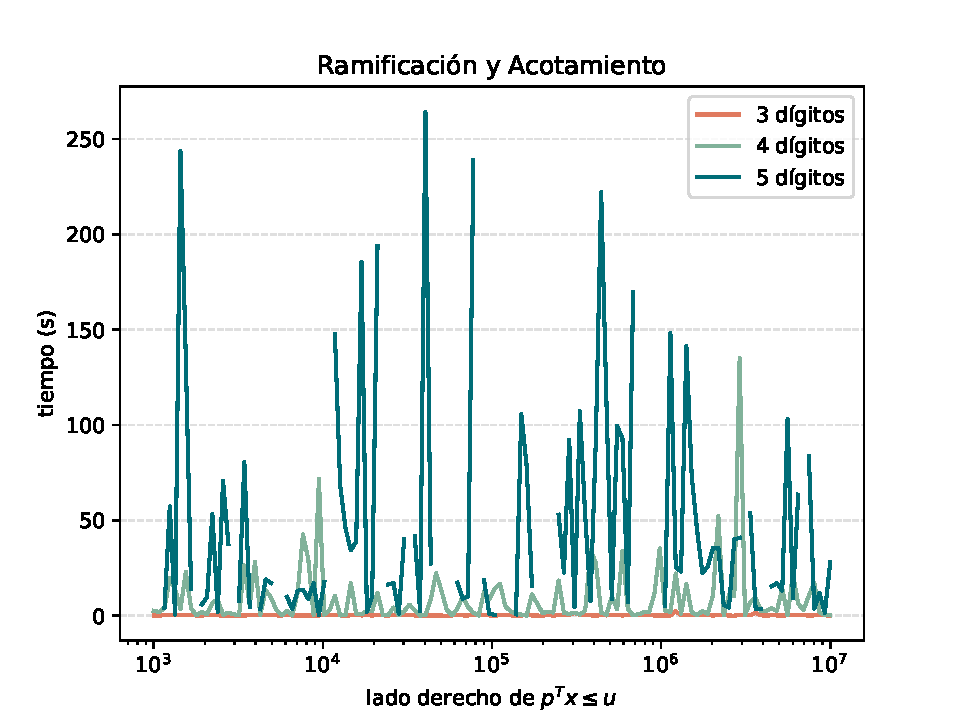
\includegraphics[width=\linewidth]{/home/tempdata/repos/thesis/static/inf/digits-bb_full.pdf}
  \end{subfigure}
  \hfill
  \begin{subfigure}{0.80\textwidth}
    \centering
    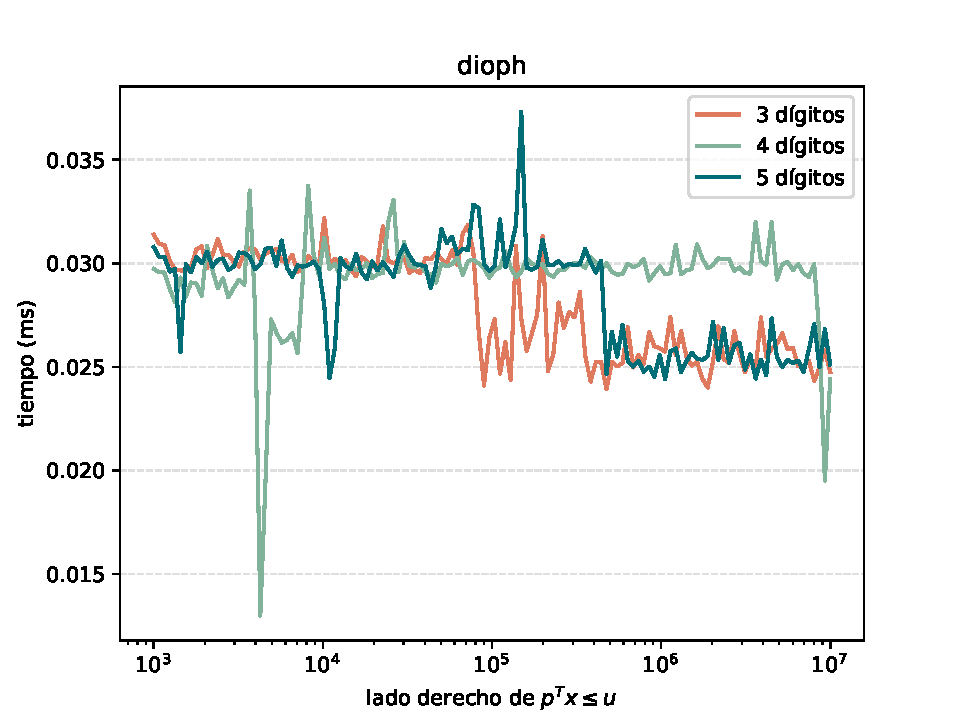
\includegraphics[width=\linewidth]{/home/tempdata/repos/thesis/static/inf/digits-dioph.pdf}
  \end{subfigure}

  \caption{Tiempos de terminación promedio cuando varía el presupuesto y el
			número de digitos. \textit{Arriba}: Resultados en segundos de R\&A. \textit{Abajo}:
			Resultados en milisegundos de nuestro método \texttt{dioph}.}
  \label{fig:exp:inf:rhs}
\end{figure}

Por los resultados obtenidos en las dos subsecciones anteriores, no sorprende que el algoritmo
\ref{algo:inf} tenga mejores tiempos de terminación que R\&A, y que no se vea afectado por la
precisión numérica del vector objetivo $\vec{p}$. Esto solo muestra que los tiempos de terminación
de R\&A son lentos para instancias de \eqref{theory:formulation}.

En realidad, nos interesa mostrar la inestabilidad numérica de R\&A a medida que la precisión del
vector objetivo $\vec{p}$ aumenta. Para ello, fijamos una de las $N = 128$ instancias y dividimos el
tiempo de terminación usando $\vec{p}_4$ entre el correspondiente tiempo usando $\vec{p}_3$; si
R\&A no encontró una solución en cualesquiera de los dos problemas, nos deshacemos de este
dato. Realizamos el mismo procedimiento entre $\vec{p}_5$ y $\vec{p}_4$.

Denominamos como multiplicadores a las razones anteriores, pues representan el factor de aumento en
los tiempos de terminación de R\&A cuando utilizamos una cifra decimal adicional. La figura
\ref{fig:exp:inf:hist} muestra la distribución de estos multiplicadores, donde los recortamos a un
máximo de 100. En realidad, el multiplicador más grande fue aproximadamente 5{,}422.

De acuerdo a la subsección anterior, deberíamos esperar que la gran mayoría de los multiplicadores
se concentren alrededor de $10^{n} = 10{,}000$. No obstante, solo el 20\% de las observaciones tiene un
multiplicador de $10^2 = 100$ o mayor. Después de un conteo en los archivos de registro generados
por el \textit{solver} CBC, el autor descubrió que en \textbf{todos} los casos que R\&A encontró una
solución fue a causa de una heurística y no por el método de ramificación. Por la
dificultad del árbol que genera el problema \eqref{theory:formulation}, de acuerdo a la subsección
anterior, esto parece ser razonable.

Aún cuando las soluciones fueron obtenidas exclusivamente a través de heurísticas, en el 60\% de los
casos el multiplicador es al menos 10. Es decir, una cifra decimal adicional en $\vec{p}$ provoca, en la
mayoría de los casos, que el tiempo de terminación en R\&A sea al menos diez veces mayor.

El autor espera que lo realizado en estos experimentos numéricos muestre categóricamente que el
método de Ramificación y Acotamiento no depende solo del número de variables o de desigualdades
utilizadas. Así pues, con esto damos por concluido este capítulo y continuamos con nuestro
desarrollo del segundo caso del teorema \ref{theory:th:feasibility}. Es decir, el siguiente capítulo
analiza a profundidad el caso finito.

\begin{figure}[hbtp]
	\centering
    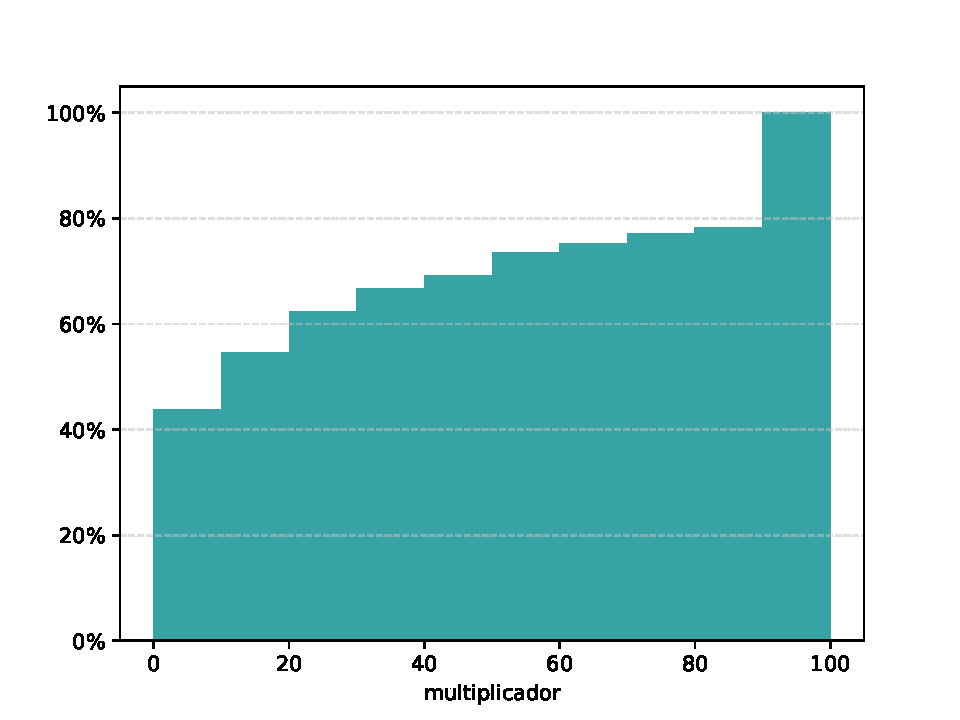
\includegraphics[width=0.9\linewidth]{/home/tempdata/repos/thesis/static/inf/mult-hist-cum.pdf}
	\caption{Distribución acumulada de los multiplicadores de tiempo.}
	\label{fig:exp:inf:hist}
\end{figure}
